\definecolor{myred}{rgb}{0.99, 0.0, 0.0}
\section{Overall Description}

\subsection{Product perspective}
\subsubsection{Scenarios}
\begin{enumerate}[label=\textbf{\Alph*}.]
    \item \textbf{Registration} \\
        Emanuele is a Computer Science and Engineering student. He wants to showcase and develop his programming skills. He heard about CKB and decides to give it a try. He goes to the CKB website and creates an account providing his personal info, his academic status (student/educator),  and setting up a password. After that, he can join tournaments and finally start showing off his abilities while becoming a code master in the process.\\
    \item \textbf{Tournament creation} \\
        Matteo is a Google hiring manager. He is looking for new talented and enthusiastic software engineers. He creates a new tournament specifying the deadline for the subscription and grants his team permission to create new battles. Users who enabled notifications will receive an email notifying them about the creation of this new tournament. Matteo finds a lot of passionate coders and engages with them in a wide variety of battles. He can then pick those who performed brilliantly and can offer them a job at Google.\\
    \item \textbf{Battle creation} \\
        Giuseppe is a recruiter from Google with an 'educator' account in CKB. He has been granted permission to create battles  by his superior, Matteo. He publishes the code kata (that includes everything to make the battle work, from the description to test cases and automation scripts) and chooses edits the battle configuration settings such as minimum and maximum number of students per team, submission deadline and more. Students subscribed to this tournament can form teams and start working on the project. After the submission deadline, teams will receive an automatic evaluation. Giuseppe is allowed to review the evaluations if need be, and finally publish the final grades for each team.  \\ 
        \textcolor{red}{\textbf{non mi è chiaro se solo chi ha creato la battaglia può rivedere i punteggi
        o anche chi ha creato il torneo o comunque altre persone con gli accessi}}\\
    \item \textbf{Badge creation} \\
        Matteo wants to add achievements to his tournament to hype up the students. He chooses a few conditions that he finds interesting selects the titles and creates the badges. At the end of the tournament, all the system checks the badges conditions to each user. Ultimately, the badges will be assigned to the students and they will be able to show them in their personal profile.
\end{enumerate}

\subsubsection{Class diagram}
The presented UML class diagram illustrates a conceptual, high-level model of the software. Due to its nature, it might model entities that won't necessarily be part of the final system under development. At this stage, it lacks references to methods and other low-level details, as these will be elaborated during the subsequent design phase.
\begin{figure}[H]
      \centering
      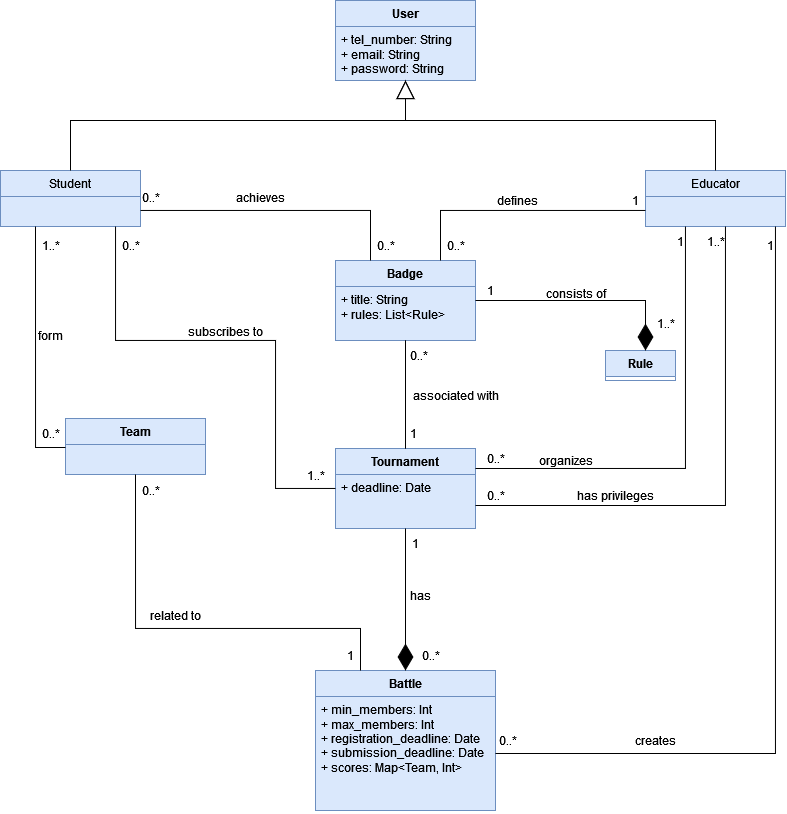
\includegraphics[scale=0.4]{src/class_uml.png}
\end{figure} \vspace{1cm}

The main entities are:
\begin{itemize}
    \item \textbf{User}\\
        A user can be either a student or an educator. Users can perform different actions according to this: educators create tournaments and battles, while students join them.
    \item \textbf{Tournament}\\
        Tournaments are created by educators and students can subscribe to them. They consist of different battles. The creator of the tournament can grant other educators privileges to define battles. Each student has a score consisting of the cumulative sum of scores obtained in all battless. Badges can also be assigned to a specific tournament.
    \item \textbf{Battles}\\
        Battles are created by educators with privileges in the scope of a tournament. Numerous settings are available for customization, such as the minimum and maximum settings for a team, deadlines and more. Students subscribed to a tournament need to form a team for each battle. At the end of the battle, each team is assigned a score between 0 and 100.
    \item \textbf{Badge}\\
        Badges are gamification objects that students can collect and show off in their profile. Educators can create badges and associate them to a specific tournament. Each badge has a set of rules that students need to satisfy in order to achieve It.
\end{itemize}

\subsubsection{State diagrams}
The purpose of the following UML state diagrams is to provide additional information about the behaviour of the system. These are the scenarios that we found more interesting.

\begin{figure}[H]
      \centering
      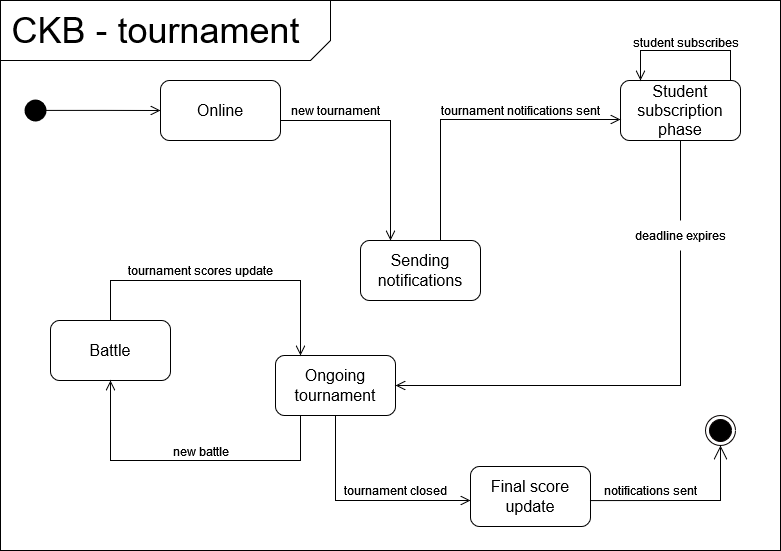
\includegraphics[scale=0.4]{src/state_diagrams/tournament_uml.png}
      \caption{Tournament timeline}
\end{figure} \vspace{1cm}
    This diagram describes what happens inside the system throughout a tournament, from the creation to the conclusion. At first, the system is waiting for new events. When an educator creates a new tournament, the system responds by sending notifications to all students. After that, the system enters a waiting state, allowing students to subscribe to the tournament until the specified deadline. When the tournament is finally open, authorized educators can create new battles. This process is seen more in-depth in the next diagram. After each battle, the system automatically updates the score for each student. New battles can be created until the creator closes the tournament. Students who took part in this tournament are sent a notification about their score, their ranking and eventual badges they may have achieved. At any moment, the creator can grant other educators permission to create battles in the scope of his tournament. \textcolor{red}{\textbf{è vero?}}\\

\begin{figure}[H]
      \centering
      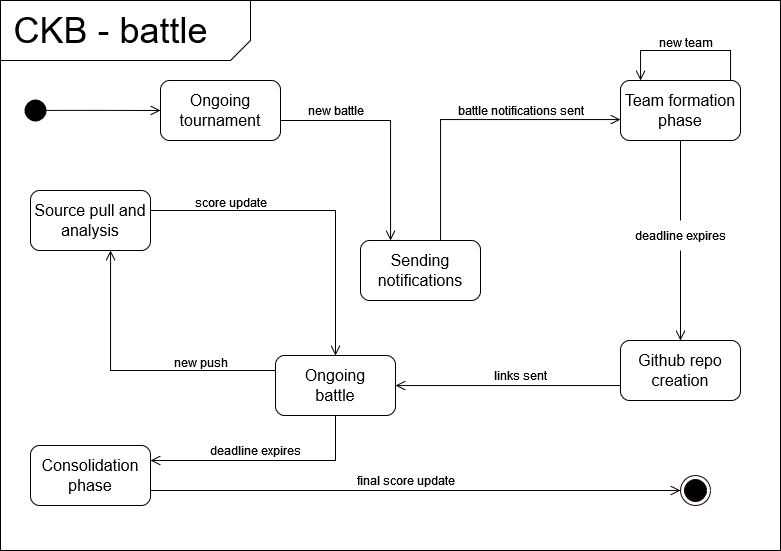
\includegraphics[scale=0.4]{src/state_diagrams/battle_uml.png}
      \caption{Battle timeline}
\end{figure} \vspace{1cm}
    This diagrams describes the steps of a battle. When a new battle is created in the scope of a tournament, the system sends a notification to all students subscribed to that tournament. Students have some time to form teams and after the deadline, a github repository is automatically created. Teams can then start working on the project. The system is notified through API calls every time a team pushes new code. Following each push, the system downloads and evaluates the sources, then publishes the scores up to that point. The specifics of these calls are beyond the scope of this diagram. After the deadline, there is a consolidation phase, where authorized educators can manually adjust the scores if need be. Finally, the battle officially ends and the students are notified.

